\documentclass[twoside,twocolumn]{article}

%\usepackage{blindtext} % Package to generate dummy text throughout this template 

\usepackage[sc]{mathpazo} 
\usepackage[T1]{fontenc} % Use 8-bit encoding that has 256 glyphs
\usepackage[utf8]{inputenc}% accents

\usepackage[english]{babel} % Language hyphenation and typographical rules

\usepackage[hmarginratio=1:1,top=20mm,columnsep=17pt]{geometry} % Document margins
\usepackage[hang, small,labelfont=bf,up,textfont=it,up]{caption} % Custom captions under/above floats in tables or figures
\usepackage{booktabs} % Horizontal rules in tables


\usepackage{enumitem} % Customized lists
\setlist[itemize]{noitemsep} % Make itemize lists more compact

\usepackage{abstract} % Allows abstract customization
\renewcommand{\abstractnamefont}{\normalfont\bfseries} % Set the "Abstract" text to bold
\renewcommand{\abstracttextfont}{\normalfont\small\itshape} % Set the abstract itself to small italic text

\usepackage{titlesec} % Allows customization of titles
\renewcommand\thesection{\Roman{section}} % Roman numerals for the sections
\renewcommand\thesubsection{\roman{subsection}} % roman numerals for subsections
\titleformat{\section}[block]{\large\scshape\centering}{\thesection.}{1em}{} % Change the look of the section titles
\titleformat{\subsection}[block]{\large}{\thesubsection.}{1em}{} % Change the look of the section titles

\usepackage{fancyhdr} % Headers and footers
\pagestyle{fancy} % All pages have headers and footers
\fancyhead{} % Blank out the default header
\fancyfoot{} % Blank out the default footer
\fancyhead[C]{FIR coefficients from cardinal sinus $\bullet$ November 2016 } % Custom header text
\fancyfoot[RO,LE]{\thepage} % Custom footer text

\usepackage{titling} % Customizing the title section

\usepackage{hyperref} % For hyperlinks in the PDF
\usepackage{amsmath} % Customizing the title section
\usepackage{graphicx,epstopdf}
\usepackage{mathtools}
%----------------------------------------------------------------------------------------
%	TITLE SECTION
%----------------------------------------------------------------------------------------

\setlength{\droptitle}{-4\baselineskip} % Move the title up

\pretitle{\begin{center}\Huge\bfseries} % Article title formatting
\posttitle{\end{center}} % Article title closing formatting
\title{Using cardinal sinus signal to generate FIR filters } % Article title
\author{%
\textsc{Samuel Dupont}\\ %\thanks{A thank you or further information} \\[1ex] % Your name
%\normalsize Université du Maine \\ % Your institution
\normalsize \href{mailto:Samuel.dupont.etu@univ-lemans.fr}{Samuel.dupont.etu@univ-lemans.fr } 
}

\date{November 06, 2016 \\ Last update: \today}
\renewcommand{\maketitlehookd}{%
\begin{abstract}
\noindent 
A recap to generate FIR filter coefficients using cardinal sinus. It encompasses different filters : low-pass, high pass and bandpass. A such method is useful to generate the coefficients in embedded system in a versatile way, the program calculating the coefficients automatically. However this method as the draw back of necessitating a great number of points which lead to a slow paced filter. The matlab program used to implement the different FIR filter can be found on the following link: \href{https://github.com/Nuopel/Filtering}{Link to program}
\end{abstract}
}

%----------------------------------------------------------------------------------------

\begin{document}

% Print the title
\maketitle


\section{Introduction}
It's quite easy to understand that the ideal filter in frequency term is a step, such that from the drop of the step there is no more signal, as shown on Figure \ref{step}.\\
Then, it's well known in signal processing that the Fourier transform of a step or rectangular window is a cardinal sinus ($sinc$), in the other way around a $sinc$ in the time domain gives a rectangular shape in the Fourier domain, if written it gives the equation \ref{eq:sinctime}. 
\begin{equation}
	\begin{split}
		h(t)=F^{-1}\lbrace H(f) \rbrace & =  \frac{sin(\pi f_c t)}{\pi t}\\
										& =  f_c\  sinc(\pi f_ct),
	\end{split}
\label{eq:sinctime}
\end{equation} 
with,
\begin{equation}
H(f)=rect(\frac{f}{f_c}),
\label{eq:rect}
\end{equation} 
the normalised cut off frequency denoted as:
\begin{equation}
f_c=\frac{2f_c}{f_s},
\end{equation} 
$f_s$ being the sampling frequency, $f$ the frequency, $t$ the index of the abscissa.\\
An illustration of the cardinal sinus can be seen on Figure \ref{sinc}. 
\begin{figure}[h!]
	\centering
	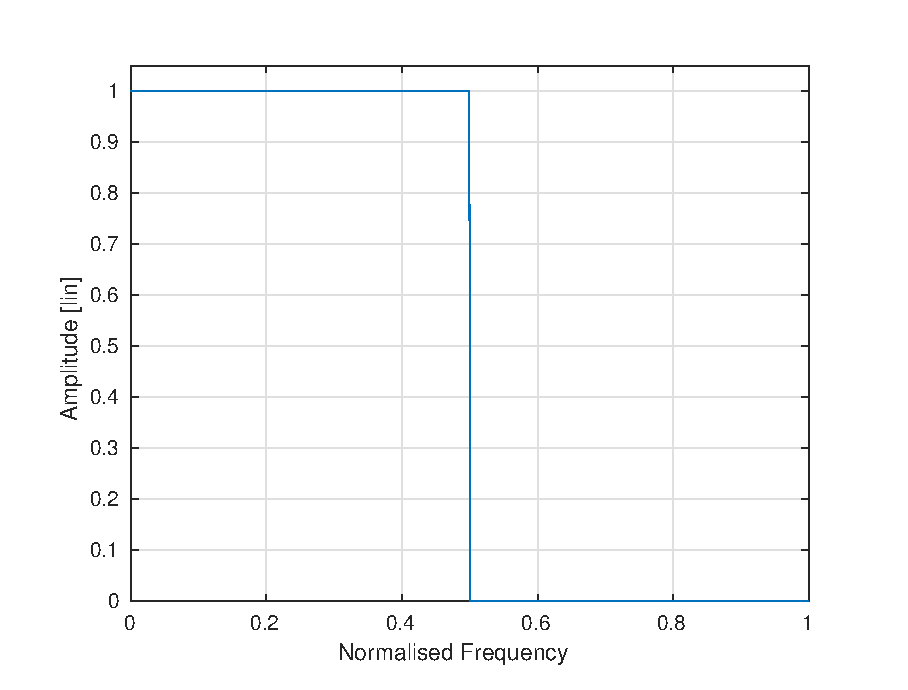
\includegraphics[scale=0.45]{./images/step.eps}
	\caption{Normalised step, $f_c=0.5$}
	\label{step}
\end{figure}
\begin{figure}[h!]
	\centering
	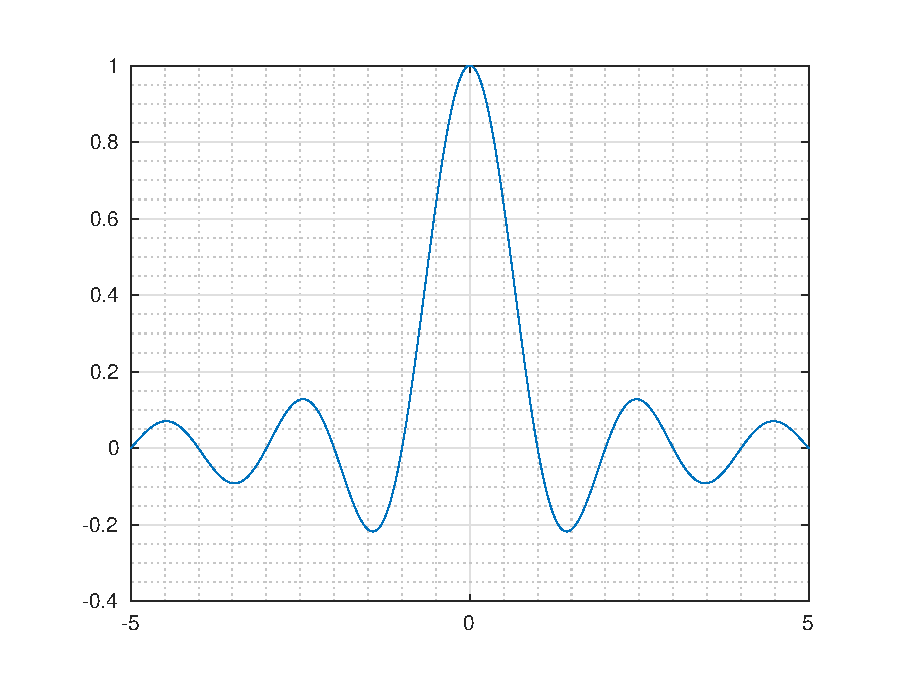
\includegraphics[scale=0.45]{./images/normalised_sinus.eps}
	\caption{Normalised cardinal sinus, $f_c=1$}
	\label{sinc}
\end{figure}

\section{Methods}

It's not possible to have an infinite number of coefficients, thus in order to implement FIR filter it's required to sample and window it.  This lead in the discrete world with all the problems of aliasing, maximum frequency...\\ \\ The number of coefficients in the filter is often critical as the more there is the slower will be the response time, but if there is not enough the frequency response will be badly impacted (further explanation in section V.\ref{influ}) . \\


\subsection{FIR filter implementation}
The Figure \ref{discrete_sinc} shows the weight coefficients of a 31 points low-pass filter obtained from equation \ref{eq:sinctime}.\\ It can be seen  that -6dB is attained (0.5) for the desired cut of frequency. The linear frequency response highlight the ripples which are generated by the truncation of the infinite $sinc$ to a finite number.\\ It's possible to reduce this ripple by windowing the signal.\\ The filters are shown from $-\frac{N}{2}$ to $\frac{N}{2}$ in order to show the filter in a centred way, however when filtering the first coefficient correspond to  $-\frac{N}{2}$. When implementing $n$ goes from $1$ to $N+1$ or $0.5$ to $N+0.5$, if even and odd number of $N$ respectively.
\begin{figure}[h!]
	\centering
	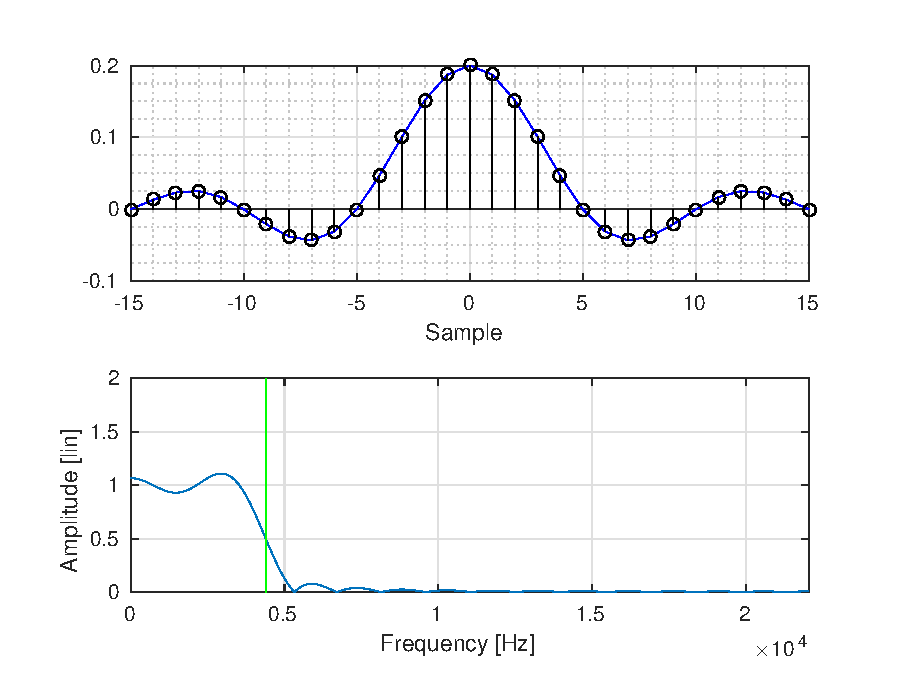
\includegraphics[scale=0.45]{./images/lp_31pts_fc02.eps}
	\caption{Low-pass, 31 coefficients, obtained from a cardinal sinus and its frequency response, $f_c=0.2=\frac{4410*2}{44100}$. The green line shows the cut off frequency.}
	\label{discrete_sinc}
\end{figure}

\subsection{Windowing}
In order to prevent the ripple induced by a low number of coefficient it's possible to window the filter. The Blackman window is took for example and is defined by the equation:
\begin{equation}
 0.452 - 0.5*cos(\frac{2\pi n}{N}) + 0.08cos(\frac{4\pi n}{N}),
\label{eq:blackman}
\end{equation}
where $n$ is the index value of the filter coefficients and $N$ the number of coefficients.\\ \\
The Figure \ref{eq:blackman} shows the previous filter and its Blackman windowed version. It can be seen that the ripple are no more present in the windowed version, the roll-off is however more fast.\\ \\
\begin{figure}[h!]
	\centering
	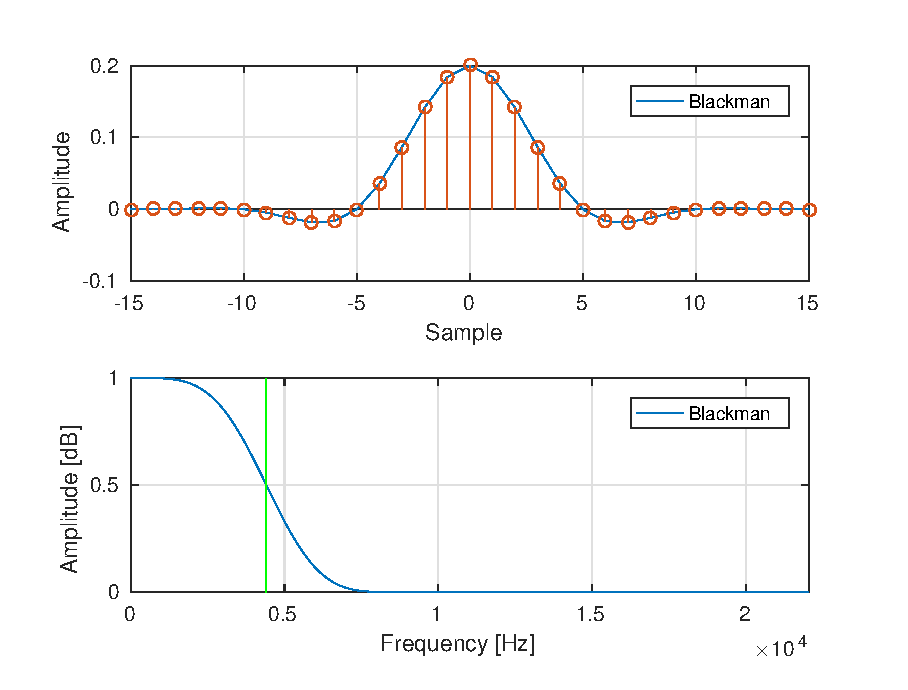
\includegraphics[scale=0.45]{./images/lp_31pts_fc02_blackman.eps}
	\caption{Low-pass 31 coefficients obtained from a	 cardinal sinus and its frequency response, $f_c=0.2$, with Blackman window.}
	\label{blackman}
\end{figure}
 There are several different types of windows, the most common are introduced in table \ref{table:tab1}, the Figure \ref{windows} is presenting their different shape, and the Figure  \ref{windowsfft} their impact on the low-pass frequency response. It can be observed from the last Figure that each windows reduce the ripple but have different roll off.
 
 \begin{table}

 	 \begin{center}

 	 	\begin{tabular}{ |l | c | }
 	 		\hline
 	 		Bartlett & $w(n)=1-\frac{2 |n-\frac{N}{2}|}{N}$ \\ \hline
 	 		Blackman &  $w(n)= 0.452 - 0.5cos(\frac{2\pi n}{N})$ \\
 	 		& $\space \space+ 0.08cos(\frac{4\pi n}{N})$ \\ \hline
 	 		Hamming & $w(n)=0.54 - 0.456 cos(\frac{2\pi n }{N})$ \\ \hline
 	 		Hanning& $w(n)=0.5 - 0.5 cos(\frac{2\pi n }{N})$\\ \hline
 	 		Rectangular& $w(n)=1$\\ \hline
 	 		
 	 	\end{tabular}
 	 	
 	 \end{center}
	 \caption{Different common windows}
 	 \label{table:tab1}

 \end{table}

\begin{figure}[h!]
	\centering
	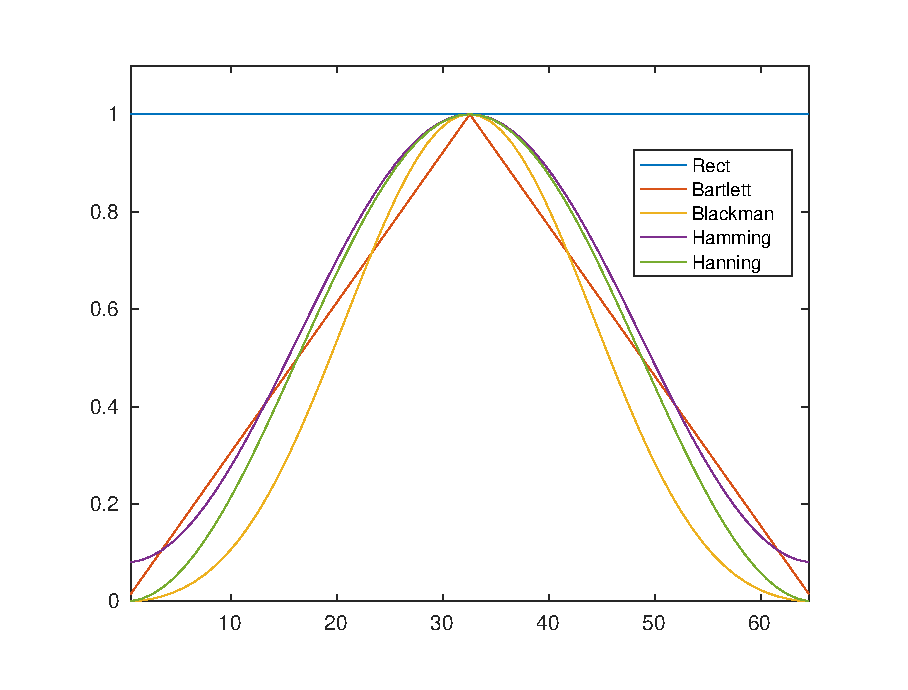
\includegraphics[scale=0.45]{./images/windows.eps}
	\caption{Different windows in time domain.}
	\label{windows}
\end{figure}
\begin{figure}[h!]
	\centering
	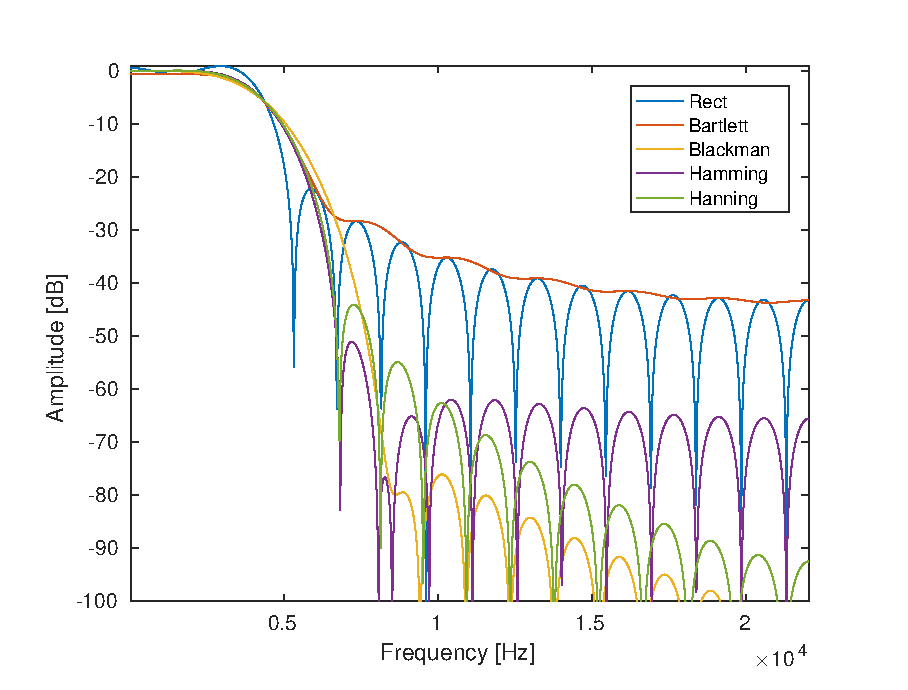
\includegraphics[scale=0.45]{./images/windows_fft.eps}
	\caption{Different windows applied to a low-pass filter $f_c=0.2$.}
	\label{windowsfft}
\end{figure}

\section{Other kind of Filters}
\subsection{High-pass filter}
The high-pass filter can be constructed using the low-pass filter. Indeed it just needed to let pass all the frequencies that are stopped by the low-pass and stop the ones that it lets	 pass. For the sake of this result it can be used the spectral inversion explained on the following equations, departing from the frequency domain.\\
\begin{equation}
H_{hp}[f]=1-H_{lp}[f],
\end{equation}
then, using the inverse Fourier transform:
\begin{equation}
F^{-1}\lbrace H_{hp}[f] \rbrace=\sigma[n]-H_{lp}[n],
\end{equation}
where $\sigma[n]$ is the Dirac impulse.\\ \\
In the end  in order to implement the high-pass filter it needed to inverse the sign of the low-pass and to set the center of the filter	$h_{hp}[n_c]$ to $1-h_{lp}[n_{c}]$.\\
The equation is written as follow (even number $N$):
\begin{equation}
h_{hp}[n]=
\left\{
\begin{aligned}
-f_c\  sinc(\pi f_cn) \ \text{if}\ n\neq \frac{N}{2} \\
1-f_c \ \text{if}\ n=\frac{N}{2}\\
\end{aligned}
\right.
\end{equation}

The figure \ref{highpass} shows the time and frequency domain of a high pass filter. In the time domain the spectral inversion is easily observable by it's peak at 0.
\begin{figure}[h!]
	\centering
	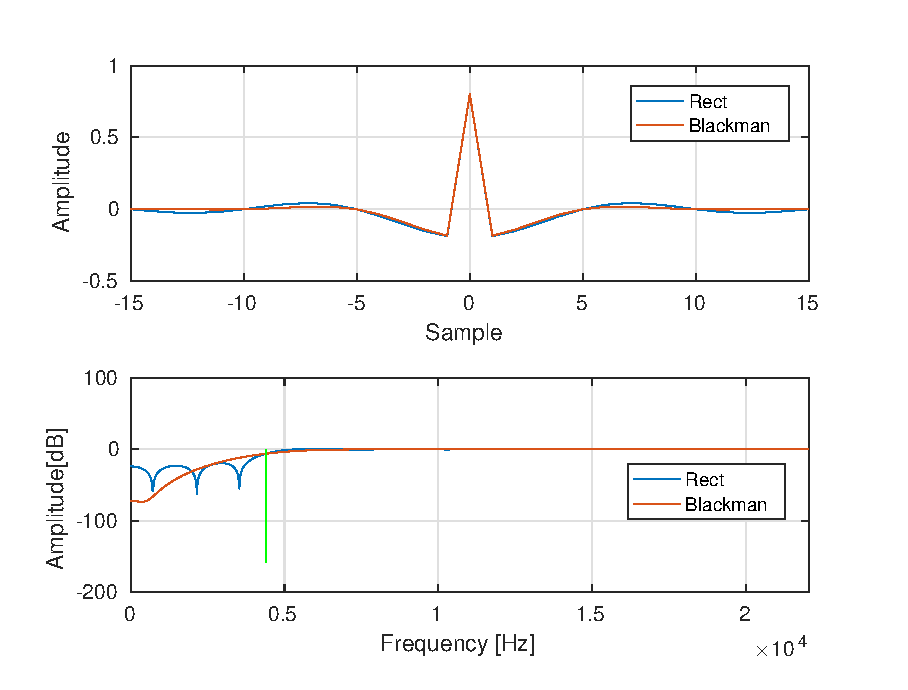
\includegraphics[scale=0.5]{./images/highpass.eps}
	\caption{High-pass filter 31 coefficients $f_c=0.2$, with and without Blackman windows.}
	\label{highpass}
\end{figure}
\subsection{Bandpass filter}
The bandpass filter is constructed from a high-pass filter and a low-pass filter. The equation can be written as follow:
\begin{equation}
	h_{bp}[n]= f_{ch}\  sinc(\pi f_{ch}n) - f_{cl}\  sinc(\pi f_{cl}n), 
\end{equation}
where $f_{cl}$ is the low cut off frequency ans $f_{ch} $ is the high cut off frequency. The Figure \ref{bandpass} show a bandpass produced.
\begin{figure}[h!]
	\centering
	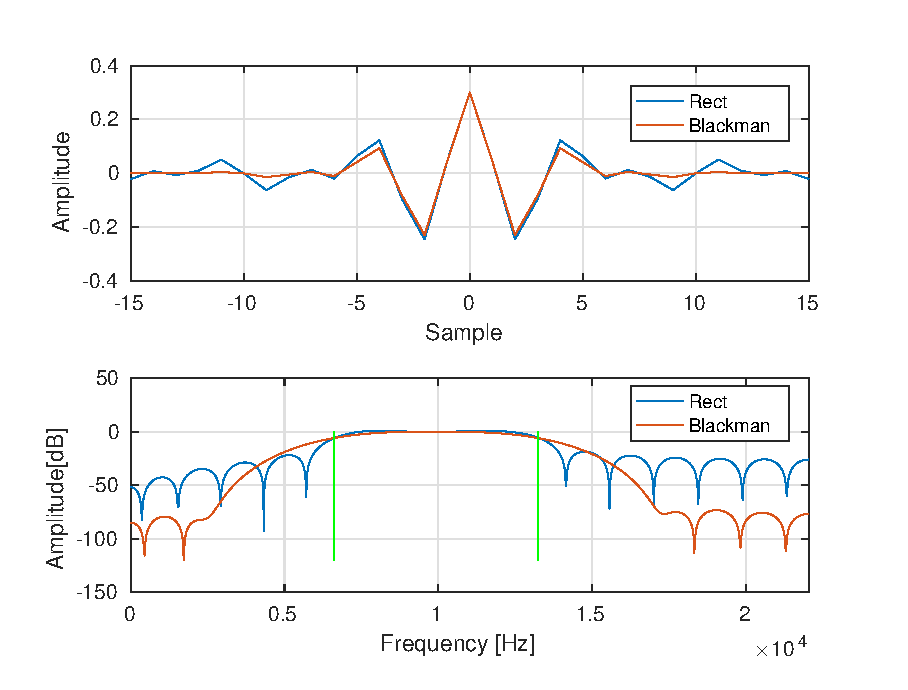
\includegraphics[scale=0.5]{./images/bandpass.eps}
	\caption{Band pass filter 31 coefficients $f_{c1}=0.3$, $f_{c2}=0.6$, with and without Blackman windows.}
	\label{bandpass}
\end{figure}

\section{Other kind of transformations}
We have seen before that the spectral inversion consist in applying a Dirac in the middle of the filter and inverting the sign of the filter. In the same way, it exists other kind of simple transformations which can applied to the filter. It will be seen  the spectral shifting and the spectral mirroring.\\ \\
 In this part the transformation will be applied on the low pass showed on Figure \ref{lowpass}, $f_c=0.2$ so 4410 Hz for a sampling frequency of 44100 Hz and 31 coefficients. 
 \begin{figure}[h!]
 	\centering
 	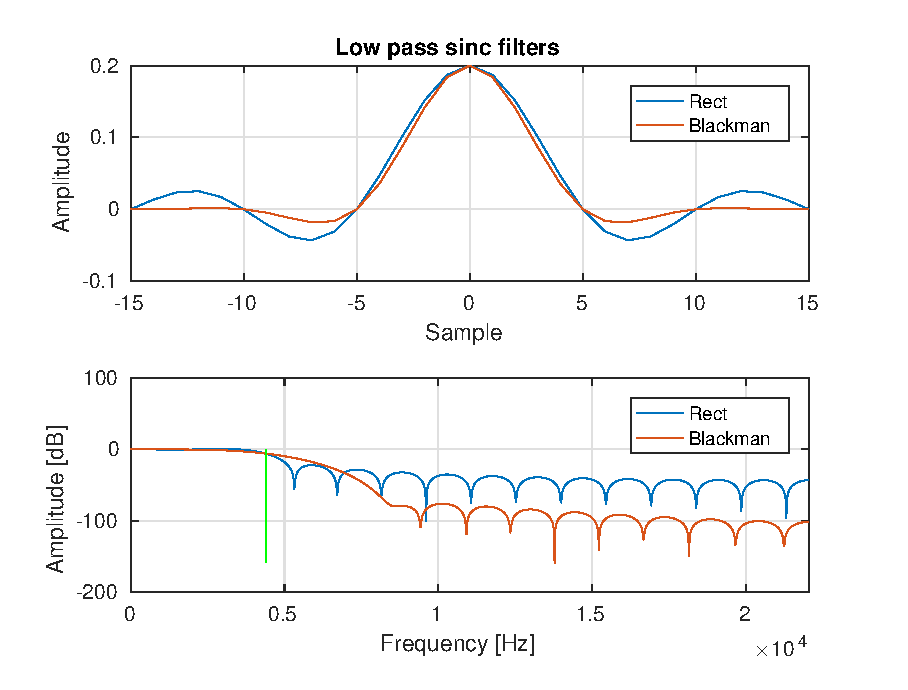
\includegraphics[scale=0.5]{./images/basetrans.eps}
 	\caption{Low-pass filter 31 coefficients $f_{c}=02$, with and without Blackman windows.}
 	\label{lowpass}
 \end{figure}
  
\subsection{Spectral shifting}
The spectral shifting is obtained by multiplying the filter by the window :
\begin{equation}
w_s[n]=cos(n\pi shift),
\end{equation}
	where the $shift$ is the normalised frequency (ex: 4000/Nyquist frequency).\\
	The shift filter is presented Figure\ref{shiftfilt}. 
	\begin{figure}[h!]
		\centering
		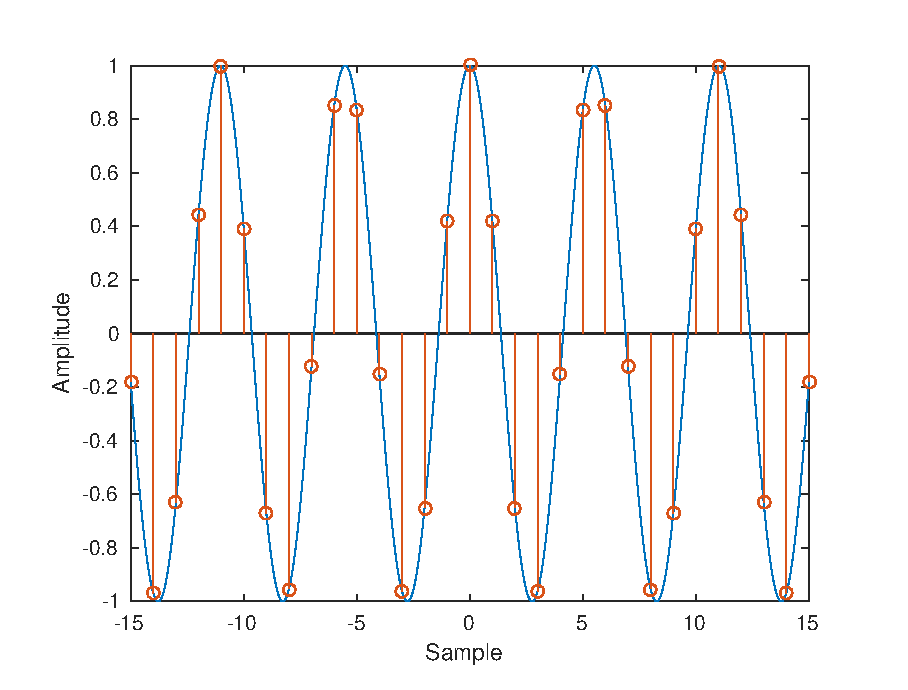
\includegraphics[scale=0.5]{./images/shiftfilt.eps}
		\caption{Shift filter used for 31 coefficients}
		\label{shiftfilt}
	\end{figure}
This effect shift the negative frequencies in the positive part of the spectrum, which mean that if the shift is to important the negative cut off will appear in the positive part at $shift-f_c$, as shown in Figure \ref{shifted}. 

\begin{figure}[h!]
	\centering
	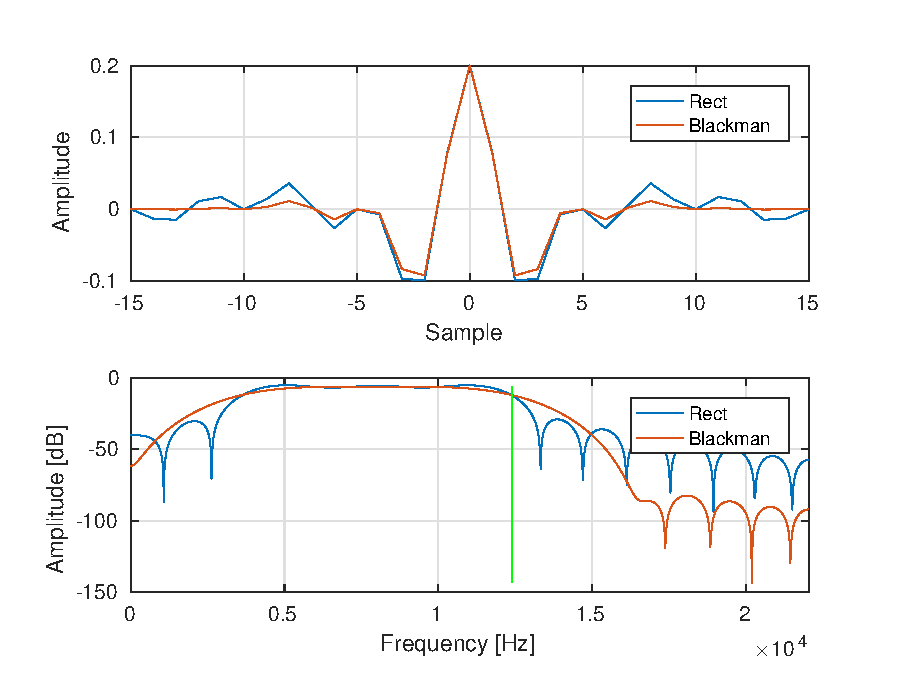
\includegraphics[scale=0.5]{./images/shifted.eps}
	\caption{Low-pass shifted filter 31 coefficients $f_{c}=0.2$, with and without Blackman windows,green line at $f_c+8000*2/f_s$.}
	\label{shifted}
\end{figure}


\subsection{Spectral mirroring}

The spectral mirroring is obtained by using a filter consisting of alternated positive and negative impulse as shown on Figure \ref{mirrorfilt}. The filter applied on the low pass will give a high-pass with a new $f_{cmirror}=1-f_c$ as shown on Figure \ref{mirrored}.
\begin{figure}[h!]
	\centering
	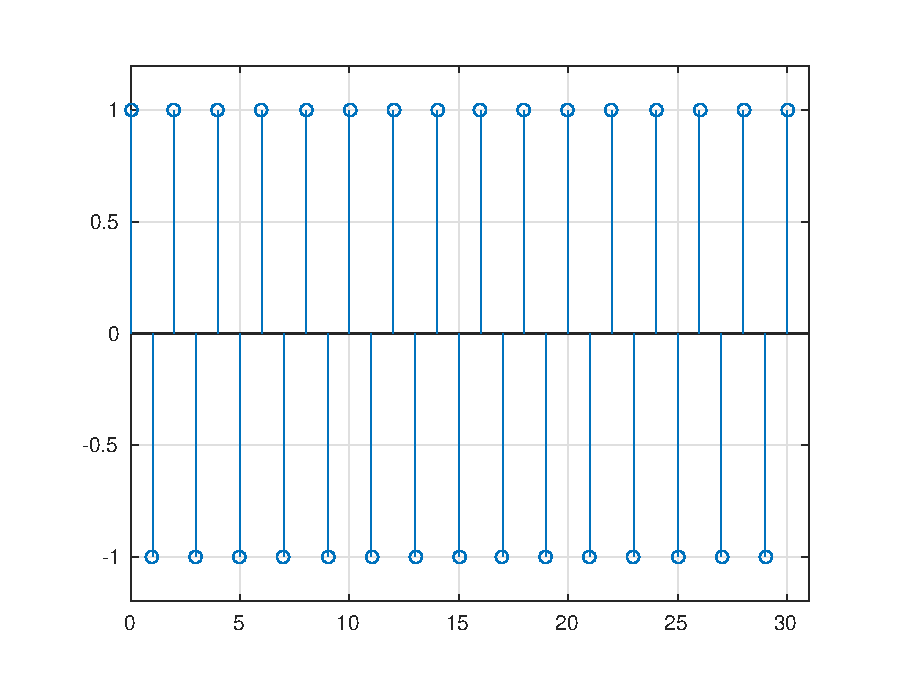
\includegraphics[scale=0.5]{./images/mirrorfilt.eps}
	\caption{Mirror filter used for 31 coefficients}
	\label{mirrorfilt}
\end{figure}

\begin{figure}[h!]
	\centering
	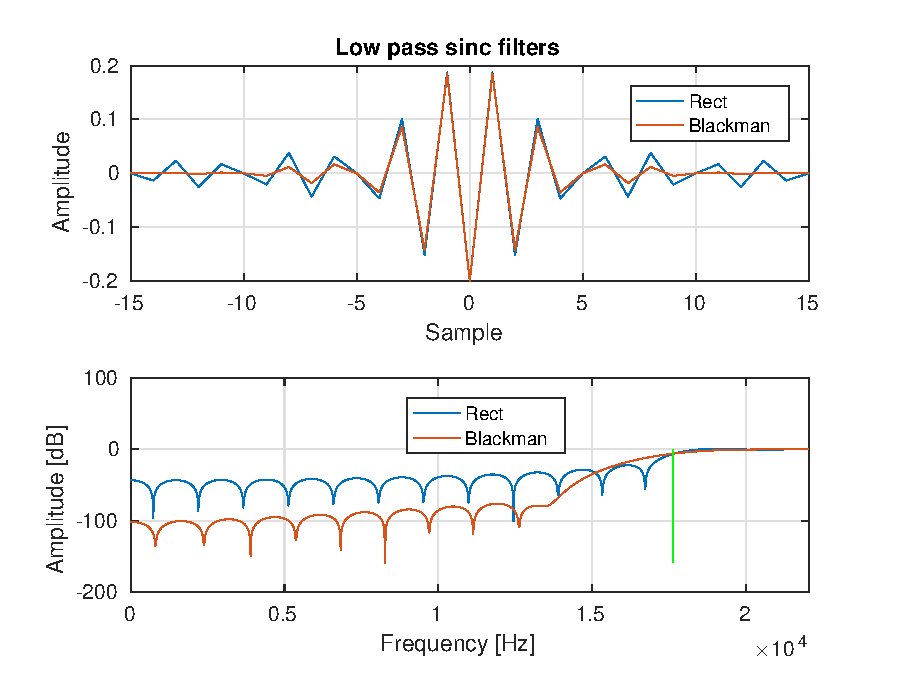
\includegraphics[scale=0.5]{./images/mirrored.eps}
	\caption{Low-pass 31 coefs, mirrored with and without Blackman windows. Green line at Nyquist frequency minus $f_c=0.2$}
	\label{mirrored}
\end{figure}


\section{Code implementation of the filters}
\label{sec:code}
This part will not discuss of code in itself but rather in the thing that it need to be paid attention during the implementation, especially about the number of coefficients influence and how to implement in case of odd or even numbers, what does it imply.

\subsection{Influence of points numbers}
\label{influ}
 In time domain it's obvious that the filter will just be longer if there are more points, the cardinal sinus being truncated with a bigger window...\\ \\
The influence on the frequency is illustrated by the Figure \ref{influence}, where it can be seen that the more points is it the more accurate will be the rectangle reconstruction in frequency domain.\\ \\ This accuracy in frequency imply a long and slow filter implementation as numerous operation will be needed to apply this filter to the signal, this is the so called duality time/frequency in signal processing.

\begin{figure}[h!]
	\centering
	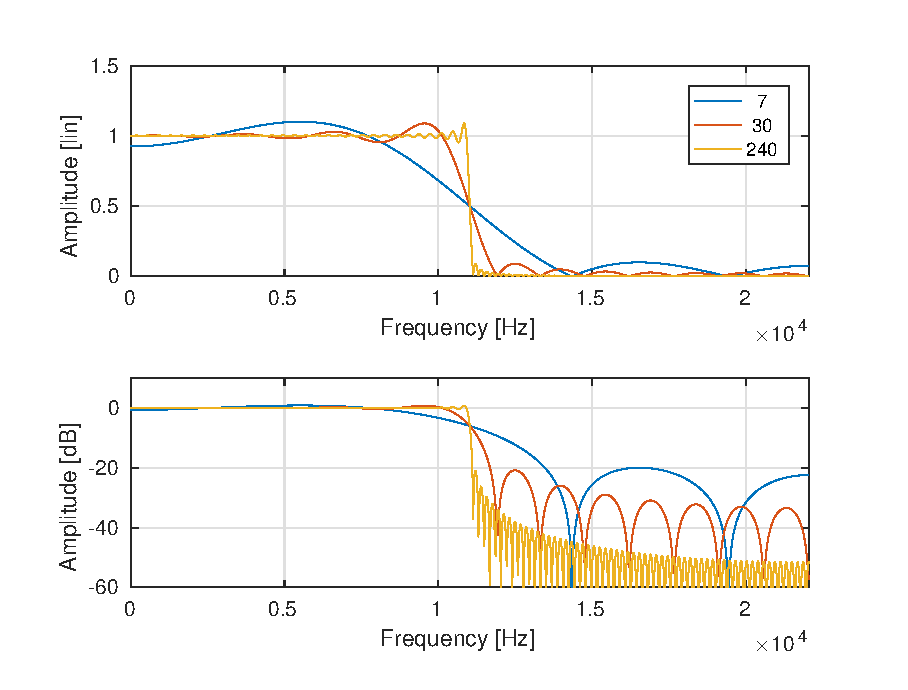
\includegraphics[scale=0.5]{./images/pt_influence.eps}
	\caption{Linear and dB frequency response of low-pass sinc filters $f_c=0.5$ with 7,30 and 240 points }
	\label{influence}
\end{figure} 

\subsection{The trap of odd and even points}
It's totally possible to implement a odd or an even tap number for the filter, it's just needed to define how the filter will be organised.\\ \\
For odd number it's quite simple, the center is defined they will be even number on each side of the center.\\
For even number,  I choose by analogy to the fft to set the center in the left part (as if it's the positive part), thus there will be one more coefficient in the FIRst half as there is the center in the second half.\\ \\

Ok, nothing difficult until there. But now with the windows to avoid ripple? They need to be aligned to the center of the filter (center=peak of the sinc), else it will slightly damage the filter.\\
Then how to achieve this? Actually, all the previous windows are based on a ratio of $n$ over $N$, the trick is just that $n$ at the center of the filter is equal to $\frac{N}{2}$ so that the ratio at the center is 0.5:
\begin{itemize}
	\item for odd tap number, $n$ must begin at 0.5 and finish at $N+0.5$ ,
	\item for even tap number, $n$ begin a 1 so that the center is well situated at $\frac{N}{2}+1$.
\end{itemize}

\section{Conclusion}
This article shows a recap to realise different FIR filter based on cardinal sinus filter, due to the limitation induced by the truncation a set of windows are proposed to reduce the ripple. It been seen that it needed an important number of points in order to achieve the desired step frequency however this imply a slow filter at the implementation. If speed is an issue IIR filter should be considered.
%----------------------------------------------------------------------------------------
%	REFERENCE LIST
%--------------------------------------%
\begin{thebibliography}{99} % Bibliography - this is intentionally simple in this template

\bibitem[\href{http://www.labbookpages.co.uk/audio/firWindowing.html}{http://www.labbookpages.co.uk/audio/firWindowing.html}]{site1}
\bibitem[\href{http://www.phon.ucl.ac.uk/courses/spsci/dsp/filter.html}{http://www.phon.ucl.ac.uk/courses/spsci/dsp/filter.html}]{site2}
\bibitem[\href{http://www.eetimes.com/document.asp?doc\_id=1275863}{http://www.eetimes.com/document.asp?doc\_id=1275863}]{site3}

%\newblock Assortative pairing and life history strategy - a cross-cultural
%  study.
%\newblock {\em Human Nature}, 20:317--330.
 
\end{thebibliography}--------------------------------------------------



%----------------------------------------------------------------------------------------

\end{document}
